\documentclass[notuble,10pt,a4paper]{leaflet}
\usepackage{color}
\usepackage{flowfram}
\usepackage{graphicx}
\usepackage{wrapfig}
\usepackage{hyperref}
\usepackage{rotating}
\usepackage{multirow}
\usepackage{array}
\pagestyle{empty}
\usepackage{multirow}
\usepackage{titlesec}
\usepackage[usenames,dvipsnames]{xcolor}
\titleformat*{\section}{\color{Blue}}
%\newenvironment{tips}
%{
%\noindent
%\begin{table}
%\begin{center}
%\begin{tabular}{m{.2cm} m{\textwidth}}
%\rotatebox{90}{\textbf{\resizebox{0.45\textwidth}{!}{FISAT}}}&
%}
%{\end{tabular}
%\end{center}
%\end{table}
%\bigskip
%}

%FONT Change
%\renewcommand{\familydefault}{cmss} 
%To Draw a horizontal Line
\newcommand{\sectionline}{
  \nointerlineskip \vspace{\baselineskip}
  \hspace{\fill}\rule{0.8\linewidth}{.7pt}\hspace{\fill}
  \par\nointerlineskip \vspace{\baselineskip}
}
%\AddToBackground{2}{\includegraphics[width=29.7cm]{bkf}}
%\AddToBackground{2}{\includegraphics[width=29.7cm]{cmy}}
% Make a border along the top of each page
\vtwotonetop{1cm}{0.6\paperwidth}{[cmyk]{0,0.91,0.92,0.41}}{topleft}%
{0.4\paperwidth}{[cmyk]{0,0.91,0.92,0.41}}{topright}

\vtwotonebottom{1cm}{0.6\paperwidth}{[cmyk]{0,0.91,0.92,0.41}}{bottomleft}%
{0.4\paperwidth}{[cmyk]{0,0.91,0.92,0.41}}{bottomright}

%\vtwotonebottom[1,6]{1cm}{0.6\paperwidth}{[cmyk]{0,0.91,0.92,0.41}}{bottomleft}%
%{0.4\paperwidth}{[cmyk]{0,0.91,0.92,0.41}}{bottomright}

\begin{document}
\begin{center}
{\large 2-Week ISTE Workshop} \\[.3cm]
\textit{on}\\[.4cm]
{\large \textbf{Introduction to Research Methodologies}}\\ [.3cm]
\textit{{\small Under the}}\\[.3cm]
{\normalsize National Mission on Education through ICT\\
(MHRD, Govt. of India)}\\[.4cm]
\textbf{{\large $25^{th}$ June - $4^{th}$ July 2012}}\\[.5cm]
{\large \textbf{Conducted by IIT Bombay}}\\[.5cm]
%\vfill
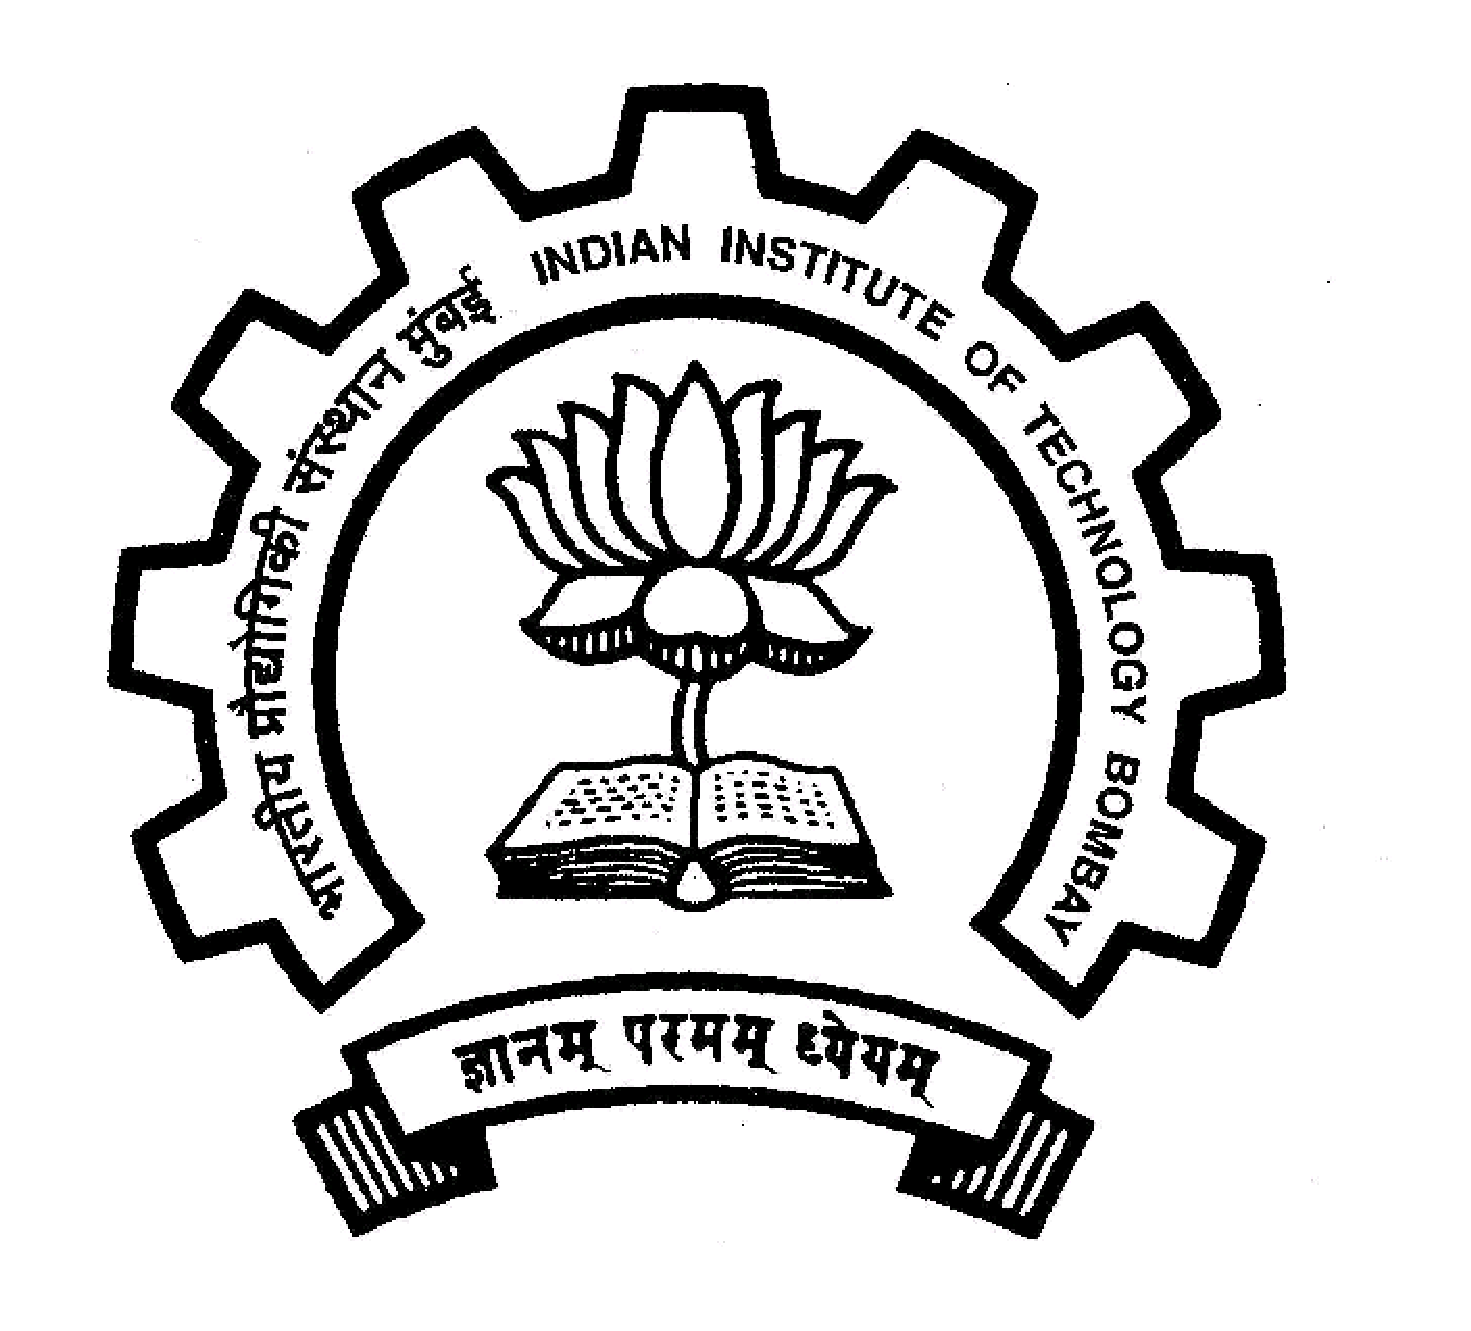
\includegraphics[scale=.15]{iitb}\\[.5cm]
\textit{{\small at}}\\[.3cm]
{\large\textbf{ Federal Institute of Science And Technology (FISAT)$^{\tiny{\mbox{TM}}}$}} \\[.4cm]

\includegraphics[scale=.13]{logod}\\
\vfill
Project Coordinator\\ 
\textbf{Prof. D.B. Phatak}\\
Dept. of Computer Science \& Engineering\\
Indian Institute of Technology Bombay\\
Mumbai – 400076
\end{center}
%\begin{titlepage}
%\title{
%}
%\vfill
%\date{}
%\author{
%\includegraphics[scale=0.2]{ffsc}\\
%\textit{at}\\
%Federal Institute of Science And Technology\\(FISAT)$^{\tiny{\mbox{TM}}}$ \\\\
%
\includegraphics[scale=.1]{logod}\\
%}
%\end{titlepage}


%\maketitle
\thispagestyle{empty} 
\newpage
\section{{\Large{2-Week ISTE Workshops conducted by IIT Bombay}}}
About 10 years ago, an important initiative was taken by IIT Bombay to enhance the teaching skills of our faculty colleagues in Engineering and Science Subjects. This initiative has now become a part of the National Mission on Education through ICT (NMEICT) supported by MHRD. We have conducted two-week ISTE workshops on Computer Programming, Database Management Systems, Thermodynamics, Basic Electronics, Heat Transfer, Software Development Techniques, Solar Photovoltaics, and Writing Effective Conference Papers. These workshops were attended by about 9,500 participating teachers across the country, at 78 remote centres, through distance mode, using the internet.
In the backdrop of the success of these workshops, we now announce a mega-workshop: a two-week ISTE workshop, on \textbf{Introduction to Research Methodologies}, to be held from \textbf{25th June to 4th July 2012, at about 200 remote Centres across the country.}
\section{{\Large How to Apply}}
Those wishing to attend this workshop should enroll online at this website: 

\url{http://www.it.iitb.ac.in/nmeict/rm}

Enrolment will be strictly online, and no other mode of applications, will be entertained. The online form contains a list of remote centres. From this list, please select up to 3 centres close to your institute, where you would wish to attend the workshop.


Last date for enrolment and for submission of permission letter is 14th June 2012.



A list of selected participants will be put up on this website on 18th June 2012. The selected participants will also be informed by email.

\emph{\textbf{LAST DATE FOR ONLINE ENROLMENT:}}
\emph{\textbf{$14^{th}$ June 2012}}
\newpage

\section{{\Large Introduction}}
Research Methodologies is being recommended by
AICTE to be a compulsory core subject for all ME/M.Tech
programmes in the country. The syllabus is currently being
drafted by a committee at AICTE. It is therefore important,
that a large number of teachers should be able to teach
this subject, or at least be fully conversant with the basic
concepts.


\section{{\Large Course Outline}}
\textit{Topics}

This course will provide an introduction to research for scientists and engineers. The goal of the course is to take a researcher through the various aspects and steps of a research project. Topics covered in the course are classified into the following main categories:
\begin{itemize}
\item Productive Thinking Skills 
\item Scientific Method and Experimentation Skills 
\item Communication Skills - Written and Oral 
\item Management of research - time management, stress management, professional ethics 
\end{itemize}

\textit{Format}

The course will consist of lectures and several interactive sessions. There will be tutorials and practical sessions wherein participants will get an opportunity to apply the research methodologies and skills discussed, to address research problems. Participants will work on several exercises individually and in teams.

\section{\Large{Course Faculty}}

\begin{itemize}
\item Prof. Shreepad Karmalkar, IIT Madras
\item Prof. Uday Gaitonde, IIT Bombay
\item Prof. Sahana Murthy, IIT Bombay
\item Prof Santosh Noronha, IIT Bombay
\end{itemize}
 
\section{{\Large Who Should Attend}}
This workshop will benefit all faculty members guiding and working on research projects in their college. We encourage teachers in the initial stages of research, such as those pursuing M.E. and Ph.D, to participate.

Limited seats may be offered \textbf{without any funding} support, to PG students to participate as observers, in case of availability of space at a remote centre.

\textbf{Note A}

Please note that the participants  will be required to make additional contributions within the following two weeks for certification. These contributions will be in the form of assignments.

\textbf{Note B}

Please note that this workshop is conducted under the eOutreach project of IIT Bombay. Live recording of the course and other created contents would be released under Open Source, through a portal. The recorded CD/DVD of the course lectures would be available for distribution at cost, to any individual/ institution. All participants are required to sign a No Objection certificate for such a release of contents contributed by them during and after the workshop. All contributors will be acknowledged.


\section{{\Large Accommodation and other support}}

Remote centres are being funded to provide tea/lunch on each day of the workshop. Accommodation may be made available for a limited number of outstation participants, but there is no guarantee. Travel expenses up to Rs.1000/- will be reimbursed against proof of actual expenditure

\section{{\Large Course Fee}}

Since  the  workshop  is  funded  by  the  National Mission on Education through ICT (MHRD, Government of India), there is \textbf{no course fee for participation}.

\newpage
\section{{\Large Eligibility}}

\begin{itemize}
\item Teachers employed in engineering colleges are eligible to attend this workshop. This includes teachers who are visiting faculty, and contract employees.
\item The participants have to submit a letter from the head of their institute stating that the participant is a bonafide employee of that institute. This letter has to be scanned uploaded on the workshop website. 
\item If the participant is unable to submit such a letter at the time of online enrolment, he/she would still be able to attend the workshop. However, he/she has to upload the letter to within 7 days after conclusion of the workshop. 
\item In case of non-submission of the letter, the participant would not be given the ISTE certificate of participation. In addition, he/she will be liable to refund the cost incurred on his/her participation.
\item Teachers from Science colleges, who are involved in research, may also apply. Such applicants will be accommodated only if there are vacant seats in the Remote Centre of their choice. If selected, their participation will also be funded to the same extent as the teachers from engineering colleges. 
\item Important: Please note that the participants will be required to make additional contributions 
within the following two weeks for certification. These contributions will be in the form of assignments.
\end{itemize}

\section{{\Large Duration and Venue}}
The two week ISTE workshop on Introduction to Research Methodologies will be conducted simultaneously at multiple remote centres across the country, in the distance mode. Every remote centre will have about 50-100 participants. The workshop will include the delivery of live interactive lectures from IIT Bombay, and locally organized tutorial and laboratory sessions. The course will be networked to the remote centres via the internet, using specially developed software called AVIEW.




\newpage

%\begin{center}
%\centering
%\includegraphics[scale=0.4]{ffsc}
%\end{center}
%\begin{center}
%\begin{tips}
%\begin{tabular}{l}
%{\resizebox{5cm}{!}{ONE}}\\ 
%{\resizebox{5cm}{!}{MILLION}}\\ 
%{\resizebox{5cm}{!}{CODES TO}} \\ 
%{\resizebox{5cm}{!}{THE COMMUNITY}}\
%\end{tabular} 
%\end{tips}
%\end{center}
%\begin{center}



\section{{\Large Remote Center}}
\textbf{Federal Institute of Science And Technology (FISAT)}, Angamaly, Kerala has been approved as one of the remote centre of this project. FISAT was established in 2002 under the aegis of Federal Bank Officers' Association Educational Society (FBOAES). The college has carved a niche for itself in education world, eloquently demonstrated by the flying colors attained by its students in academics, placements as well as in extra curricular and co-curricular activities. The campus is a class apart with magnificent infrastructure and has an ambiance that kindles creativity and encourages innovation.

The college has established research centres like Centre for High Performance Computing (CHPC), Instrumentation Research and Consultancy Centre (IRACC) and Centre for Research and Innovation in Signal Processing (CRISP) to nurture research and development. Under research promotion scheme, AICTE funded research centres were sanctioned for Signal Processing in ECE department and High Performance Computing in CSE department. 

For more details, visit \url{www.fisat.ac.in}

\section{{\Large Address for Communication}}
\textbf{Dr. Mukta Atrey}\\
Project Manager, Department of CSE,\\ 
Kanwal Rekhi Building, IIT Bombay\\
Tel.: +91-22-2576 4982/ 4983\\
Email:  \url{eoutreach@it.iitb.ac.in}

\section{{\Large Remote Center Co-ordinator}}
\textbf{Mr. Bejoy Varghese}\\
Federal Institute of Science And Technology (FISAT)\\
Hormis Nagar, Mokkanoor, Angamaly\\
Mob: +91 9446029662\\
E-mail:\url{eoutreach@fisat.ac.in}\\

\vfill
\footnotesize{\textcopyright FISAT | Prepared using \LaTeXe}



%\end{center}
\end{document}
